\documentclass[
	a4paper,
	oneside,
	DIV = 12,
	fontsize = 13pt,
	headings = normal,
]{scrartcl}

%%% Page geometry and precise margins
\usepackage[
	pass,
	left   = 20mm,
	top    = 15mm,
	right  = 10mm,
	bottom = 15mm,
]{geometry}
%%%

%%% Length calculations
\usepackage{calc}
%%%

%%% Support for color
\usepackage{xcolor}
\definecolor{lightblue}{HTML}{03A9F4}
\definecolor{red}{HTML}{F44336}
%%%

%%% Including graphics
\usepackage{graphicx}
%%%

%%% Font selection
\usepackage{fontspec}

\setromanfont{STIX Two Text}[
	SmallCapsFeatures = {LetterSpace = 5},
]

\setsansfont{IBM Plex Sans}[
	Scale = MatchUppercase,
]

\setmonofont{IBM Plex Mono}[
	Scale = MatchUppercase,
]
%%%

%%% Math typesetting
\usepackage{amsmath}

\usepackage{unicode-math}
\setmathfont{STIX Two Math}
%%%

%%% List settings
\usepackage{enumitem}
\setlist[enumerate]{
	label*      = {\arabic*.},
	leftmargin  = *,
	labelindent = \parindent,
	topsep      = 1\baselineskip,
	parsep      = 0\baselineskip,
	itemsep     = 1\baselineskip,
}

\setlist[itemize]{
	label       = {—},
	leftmargin  = *,
	labelindent = \parindent,
	topsep      = 1\baselineskip,
	parsep      = 0\baselineskip,
	itemsep     = 1\baselineskip,
}

\setlist[description]{
	font        = {\rmfamily\upshape\bfseries},
	topsep      = 1\baselineskip,
	parsep      = 0\baselineskip,
	itemsep     = 0\baselineskip,
}

%%%

%%% Structural elements typesetting
\setkomafont{pagenumber}{\rmfamily}
\setkomafont{disposition}{\rmfamily\bfseries}

% Sectioning
\RedeclareSectionCommand[
	beforeskip = -1\baselineskip,
	afterskip  = 1\baselineskip,
	font       = {\normalsize\bfseries\scshape},
]{section}

\RedeclareSectionCommand[
	beforeskip = -1\baselineskip,
	afterskip  = 1\baselineskip,
	font       = {\normalsize\bfseries},
]{subsection}

\RedeclareSectionCommand[
	beforeskip = -1\baselineskip,
	afterskip  = 1\baselineskip,
	font       = {\normalsize\bfseries},
]{subsubsection}
%%%

%%% Typographic enhancements
\usepackage{microtype}
%%%

%%% Language-specific settings
\usepackage{polyglossia}
\setmainlanguage{ukrainian}
\setotherlanguages{english, russian}
%%%

%%% Captions
\usepackage{caption}
\usepackage{subcaption}

%\DeclareCaptionLabelFormat{closing}{#2)}
%\captionsetup[subtable]{labelformat = closing}

%\captionsetup[subfigure]{labelformat = closing}

\captionsetup[table]{
	aboveskip = 0\baselineskip,
	belowskip = 1\baselineskip,
}

\captionsetup[figure]{
	aboveskip = 1\baselineskip,
	belowskip = 0\baselineskip,
}

\captionsetup[subfigure]{
	aboveskip = 0.25\baselineskip,
	belowskip = 0\baselineskip,
}

\captionsetup[subfigure]{
	labelformat = simple,
	labelformat = brace,
}
%%%

%%% Table typesetting
\usepackage{booktabs}
\usepackage{longtable}

\usepackage{multirow}

\usepackage{array}
\newcolumntype{v}[1]{>{\raggedright\arraybackslash\hspace{0pt}}p{#1}}
\newcolumntype{b}[1]{>{\centering\arraybackslash\hspace{0pt}}p{#1}}
\newcolumntype{n}[1]{>{\raggedleft\arraybackslash\hspace{0pt}}p{#1}}
%%%

%%% Dingbats
\usepackage{pifont}
%%%

%%% TikZ
\usepackage{tikz}
%%%

%%% Links and hyperreferences
\usepackage{hyperref}
\hypersetup{
	bookmarksnumbered = true,
	colorlinks      = false,
	linkbordercolor = red,
	urlbordercolor  = lightblue,
	pdfborderstyle  = {/S/U/W 1.5},
}
%%%

%%% Length adjustments
% Set baselineskip to ~15pt, default is 14.5pt
% \linespread{1.034483}
% \linespread{1.068966} % ~15.5pt
\setlength{\emergencystretch}{1em}
\setlength{\parindent}{1.5em}
\newlength{\gridunitwidth}
\setlength{\gridunitwidth}{\textwidth / 12}
\setlength{\floatsep}{1\baselineskip}
\setlength{\intextsep}{1\baselineskip}
\setlength{\textfloatsep}{1\baselineskip}
%%%

%%% Custom commands
\newcommand{\allcaps}[1]{{\addfontfeatures{LetterSpace = 5}#1}}
\newcommand{\progname}[1]{\texttt{#1}}

\newcommand{\CheckMark}{\ding{51}}
\newcommand{\Mytextrightarrow}{$\rightarrow$\hspace{0.25em}}

\newcommand{\filename}[1]{\texttt{#1}}
%%%

%%% Make typography adhere to made-up standards
\PolyglossiaSetup{ukrainian}{indentfirst = true}

% Sectioning
\RedeclareSectionCommand[
	beforeskip = -0sp,
	afterskip  = 1sp,
	indent     = 12.5mm,
	font       = {\normalsize\bfseries},
]{section}

\RedeclareSectionCommand[
	beforeskip = -0sp,
	afterskip  = 1sp,
	indent     = 12.5mm,
	font       = {\normalsize\bfseries},
]{subsection}

\RedeclareSectionCommand[
	beforeskip = -0sp,
	afterskip  = 1sp,
	indent     = 12.5mm,
	font       = {\normalsize\bfseries},
]{subsubsection}

\setlength{\parindent}{12.5mm}

\usepackage{leading}
\leading{21pt}

%%%

\begin{document}
	\newgeometry{
		left   = 20mm,
		top    = 15mm,
		right  = 10mm,
		bottom = 15mm,
		footskip = \baselineskip, % reduce footer vertical skip so page numbers are visible
	}
\setlength{\gridunitwidth}{\textwidth / 12}
	\begin{titlepage}
		\begin{center}
			Міністерство освіти і науки України\\
			Національний авіаційний університет\\
			Навчально-науковий інститут комп'ютерних інформаційних технологій\\
			Кафедра комп'ютеризованих систем управління

			\vspace{\fill}
				Лабораторна робота №5\\
				з~дисципліни «Діагностика та~експлуатація комп'ютера»\\
				на~тему «Лікування комп'ютера від~вірусів»\\

			\vspace{\fill}

			\begin{flushright}
				Виконав:\\
				студент \allcaps{ННІКІТ}\\
				групи СП-325\\
				Клокун В.\,Д.\\
				Перевірив:\\
				Масловський Б.\,Г.
			\end{flushright}

			Київ 2018
		\end{center}
	\end{titlepage}

	\section{Ціль роботи}
		Ознайомлення з~процесом використання антивірусного програмного забезпечення для~очищення комп'ютера від~вірусних загроз.

	\section{Короткі теоретичні відомості}
		При постійному контакті комп’ютера з~файлами та~носіями, які були створені або~знаходились у~інших комп’ютерах виникає ризик занесення на~свій комп’ютер програми, яка може погіршити роботу комп’ютера та~пошкодити дані на~жорсткому диску. Такі програми прийнято називати «комп’ютерними вірусами». Про комп’ютерний вірус можна сказати, що~це комп'ютерна програма, яка має здатність до~прихованого саморозмноження, одночасно зі~створенням власних копій віруси можуть завдавати шкоди: знищувати, пошкоджувати, викрадати дані, знижувати або~й~зовсім унеможливлювати подальшу працездатність операційної системи комп'ютера. 

		Розрізняють файлові, завантажувальні та макро-віруси. Можливі також комбінації цих типів. 

		Файлові віруси~— поширюється шляхом впровадження свого коду в~тіло виконуваних файлів. При кожному запуску такого зараженого файлу спочатку виконується код вірусу, і~тільки потім~— код самої програми. Об'єктом вірусного ураження можуть виступати виконувані двійкові файли~(EXE, COM), файли динамічних бібліотек~(DLL), драйвери~(SYS), командні файли~(BAT, CMD) та~інші. Заражаючи файл, вірус може потрапити до~його початку, кінця або~в~середину. Найбільш поширеним способом є~впровадження в~кінець файлу, коли його основний код дописується в~кінець файлу, а~в~початок записується команда переходу до~тіла вірусу. Щоб приховати свою присутність в~системі, файловий вірус може попередньо зберегти дату і~час останньої модифікації і~значення атрибутів файлу.

		Завантажувальні віруси~— записуються в~завантажувальний сектор дискети, твердого диска чи~флеш-накопичувача й~активізується при~завантаженні комп'ютера або~відкриття цього диску. При~звертанні до~нового диска, вірус копіює себе в~його завантажувальний сектор і~таким чином заражає його та~передається далі. Через специфіку роботи комп'ютерів майже будь-який носій, містить завантажувальний сектор, що дозволяє автоматично завантажувати розташовані на~ньому програмні коди. 

		Макро-вірус~— вірус, який написано на~мові макросів. Технічно, головною відміною макро-вірусу від~інших видів комп'ютерних вірусів є~лише середовище виконання. Для макро-вірусу таким середовищем є~не~операційна система, а~те~середовище, що~забезпечує виконання макро-програм (наприклад, мова \textenglish{Visual Basic}, що~забезпечує автоматизацію дій у~середовищі офісного пакету \textenglish{MS Office}). Зазвичай, макровірус вбудовується в~файли певних типів, для яких передбачені можливості автоматичного виконання  вбудованих в них макросів. 

		Нині відомі десятки тисяч комп'ютерних вірусів, які~поширюються через мережу Інтернет по~всьому світу. Необізнані користувачі ПК помилково відносять до~комп'\-ютерних вірусів також інші види зловмисного ПЗ~— програм-шпигунів чи~навіть спам. Такі віруси можна віднести до~типу веб-вірусів, які проникають на~інтернет-ресурси, розсилають спам та~блокують роботу серверів.

		Для боротьби з вірусами використовуються антивірусні програми або~фаерволи (мережеві екрани).

		Антивірусна програма (антивірус)~— програма для~знаходження і~лікування програм, що~заражені комп'ютерним вірусом, а~також для~запобігання зараження файлу вірусом. 

		Фаервол (\textenglish{firewall})~— тип антивірусного програмного забезпечення, що~встановлюється на~комп'ютер, сервер або~інший мережевий пристрій. Головним чином служить для~запобігання мережевих атак та~автоматичного проникнення вірусних програм на~комп’ютер. Також існують фаерволи у~вигляді фізичного пристрою, що~працюють на~прикладному рівні та~відбивають атаки, пов’язані з~фізичною природною роботи мережі.

		Сучасні антивірусні програми можуть поставлятися у~вигляді комплексних рішень, поєднуючи у~собі властивості звичайного файлового антивірусу з~можливостями програмного фаерволу.

		Також антивірусне програмне забезпечення може поділятися на~платне та~безкоштовне. Платні антивіруси, як~і~інше програмне забезпечення, потребує від~користувача оплачувати ліцензію на~використання, на~термін дії якої антивірус буде повністю захищати комп'ютер. Безкоштовні антивіруси не~вимагають витрачати гроші на~їх~використання, але в~деяких випадках можуть містити значно менше функціональних можливостей, що~негативно відображається на~захищеності комп’ютера.

		До~найбільш відомих платних антивірусних програм можна віднести:
		\begin{itemize}[noitemsep]
			\item \textenglish{Norton Antivirus/Norton Internet Security};
			\item Антивірус Касперського/\textenglish{Kaspersky Internet Security};
			\item \textenglish{ESET NOD32 Antivirus/ESET NOD32 Smart Security}.
		\end{itemize}

		Серед антивірусів з~безкоштовним використанням є:
		\begin{itemize}[noitemsep]
			\item \textenglish{avast! Free Antivirus};
			\item \textenglish{AVG AntiVirus};
			\item \textenglish{Panda Antivirus};
			\item \textenglish{Avira Free Antivirus}.
		\end{itemize}

		У~антивірусів існує два основних режими роботи: перевірка в~режимі реального часу та~перевірка за~вимогою.

		Перевірка в~режимі реального часу, або~постійна перевірка, забезпечує безперервність роботи антивірусного захисту. Полягає в~обов'язковій перевірці всіх дій скоєних іншими програмами і~самим користувачем. Перевірка відбувається на~предмет небезпечності, незалежно від~їх~вихідного виконання~— будь це свій жорсткий диск, зовнішні носії інформації, чи~інші мережеві ресурси або~власна оперативна пам'ять.

		В~деяких випадках наявності постійно працюючої перевірки в~режимі реального часу може бути недостатньо або~неможливим з~точки зору ресурсоємності. Для такого режиму зазвичай передбачається, що~користувач особисто вкаже які файли, каталоги або~області диска необхідно перевірити, а~також час, коли потрібно виконати таку перевірку~— у~вигляді розкладу або~разового запуску вручну.

		Зазвичай, після активізації, віруси копіюють свої файли у~системні теки операційної системи, через~те, що~їх~вміст невидимий для~користувача та~у~деяких випадках захищений від~втручання. До~таких тек можна віднести теки \textenglish{Windows, System32, Program Files, User} та~\textenglish{Application Data}.

		Деякі віруси створюють свої копії з~різними іменами у~різних теках створених при~роботі комп’ютера, через що~недосвідчені користувачі вважають~їх важливими системними файлами.

		Основними методами зараження вірусів є~завантаження програм та~файлів з~джерел невідомого походження, тобто використання носіїв інформації без~їх~перевірки або~завантаження маловідомих програм з~Інтернету. Останнім часом набули поширення програми, які маскуються під~завантажувальники файлів або~інші програми, запаковані у~архіви. Запуск таких програм призводить до~зараження системи і~може бути не~сприйнятий антивірусом як~небезпечна дія. У~таких випадках зловмисники підроблюють електронні підписи програм та~антивірус вважає їх~безпечними.

		Також можливе зараження комп’ютера через інтернет-браузер. Недосвідчений користувач може випадково прийняти сертифікат безпеки, який дозволить спеціально створеному інтернет-сайту завантажити на~комп’ютер вірус та~запустити його.

	\section{Хід роботи}
		Запускаємо віртуальну машину та~копіюємо пакет встановлення антивірусного програмного забезпечення та~тестовий вірусний файл на~жорсткий диск віртуальної машини. Після завершення копіювання файлів копіюємо файл з~архіву~\filename{eicar.zip} на~Робочий стіл, у~папку \verb|C:\Windows\| та~у~корінь диску~\verb|C:\|.

		Скопіювавши тестовий псевдовірусний файл, встановлюємо антивірусне програмне забезпечення. Для цього запускаємо надану програму-інсталятор «Антивірусу Касперського» та~встановлюємо антивірус відповідно до~наданих інструкцій~(рис.~\ref{fig:kaspersky-installation}).

		\begin{figure}[!htbp]
			\centering
			\begin{subfigure}{0.5\textwidth}
				\centering
				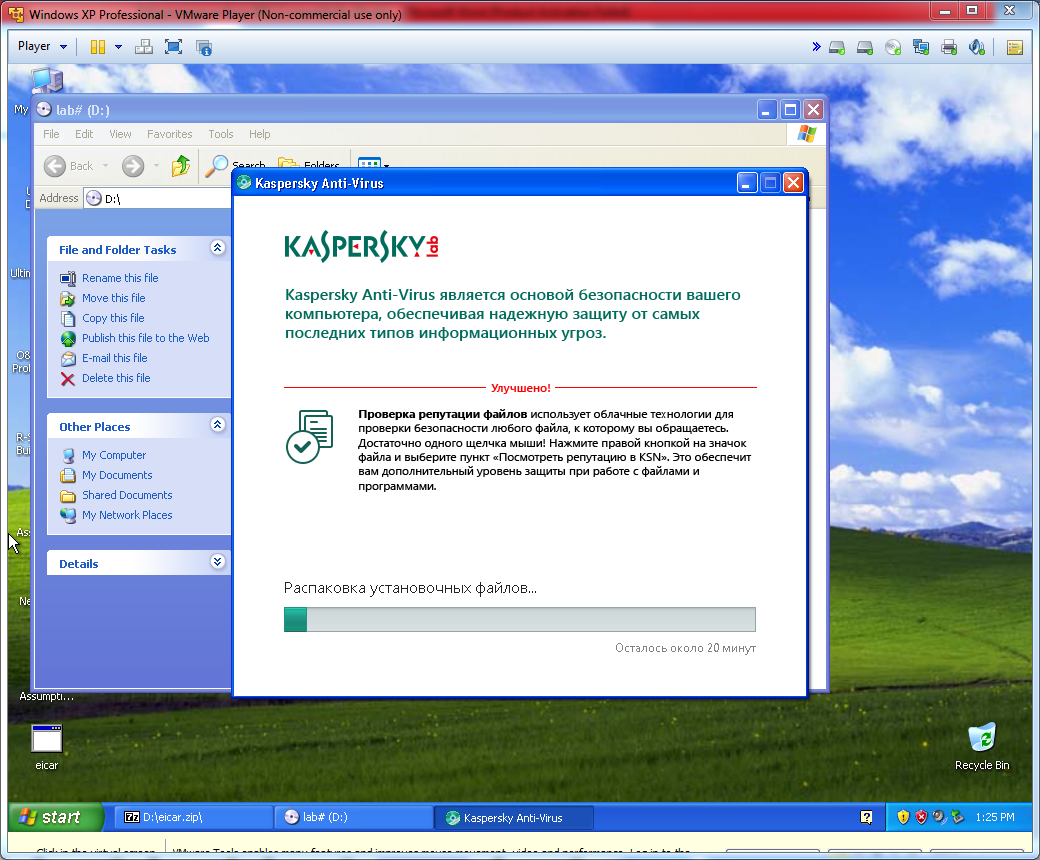
\includegraphics[height = 9\baselineskip]{./assets/y03s01-pcdiag-lab-05-p04.PNG}
				\caption{}
				\label{subfig:kaspersky-installation-start}
			\end{subfigure}%
			\begin{subfigure}{0.5\textwidth}
				\centering
				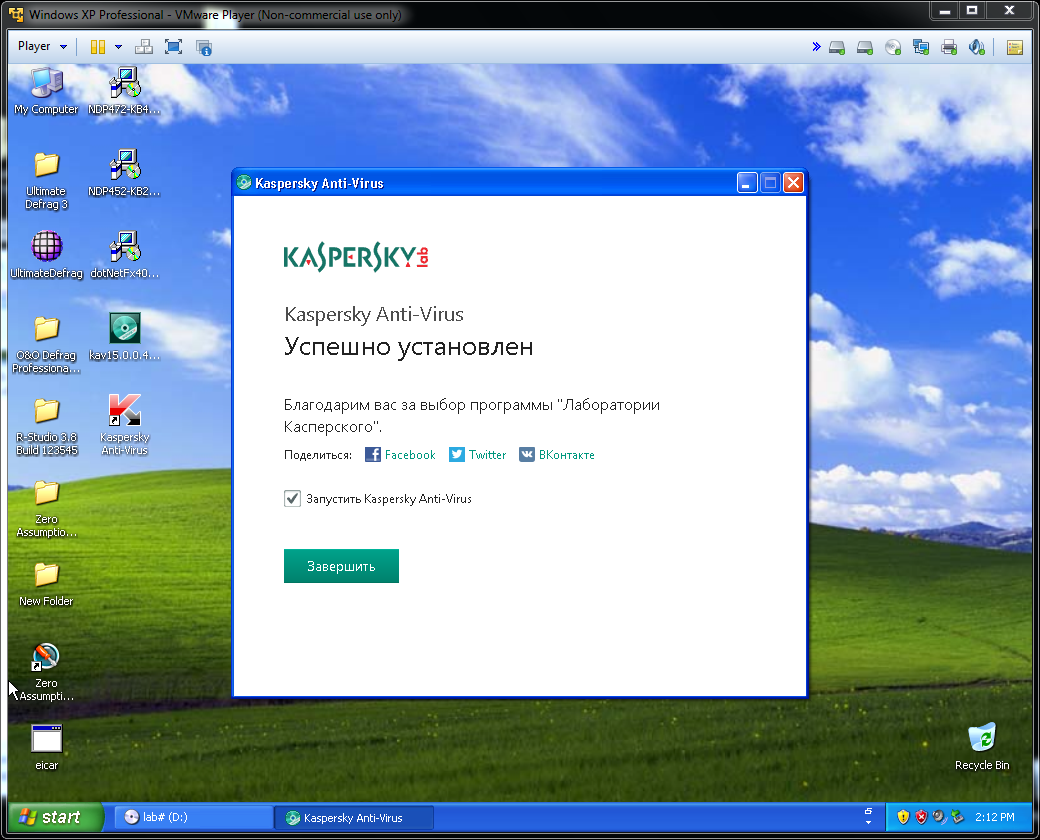
\includegraphics[height = 9\baselineskip]{./assets/y03s01-pcdiag-lab-05-p05.PNG}
				\caption{}
				\label{subfig:kaspersky-installation-finish}
			\end{subfigure}%
			\caption{Встановлення «Антивірусу Касперського»}
			\label{fig:kaspersky-installation}
		\end{figure}

		Після завершення встановлення операційна система не~запитує про~мережеву активність антивірусу, тому переходимо до~пункту оновлення баз антивірусних сигнатур. Для цього натискаємо на~кнопку «Оновлення» та~бачимо повідомлення, що~антивірусні бази неактуальні~(рис.~\ref{fig:kaspersky-signatures-update}). На~тестовій віртуальній машини відсутній доступ до~мережі Інтернет, тому оновити бази неможливо~— переходимо до~наступного пункту.

		\begin{figure}[!htbp]
			\centering
			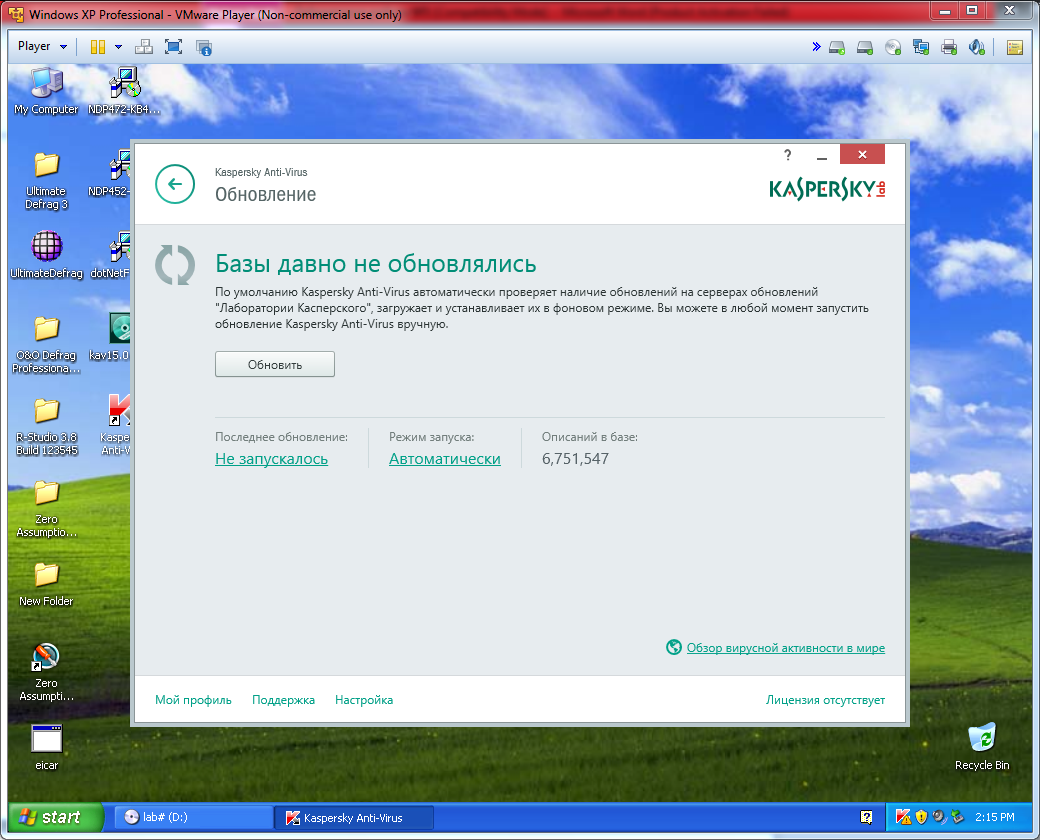
\includegraphics[height = 9\baselineskip]{./assets/y03s01-pcdiag-lab-05-p08.PNG}
			\caption{Вікно оновлення баз антивірусних сигнатур «Антивірусу Касперського»}
			\label{fig:kaspersky-signatures-update}
		\end{figure}

		Виконуємо перевірку комп'ютера на~наявність шкідливого програмного забезпечення. Для~цього відкриваємо головне меню, натискаємо кнопку «Перевірка» та~переходимо у~меню Швидкої перевірки. Однак для~економії часу на~перевірку оберемо та~запустимо Вибіркову перевірку, оскільки місцезнаходження тестового файлу нам вже відоме~(рис.~\ref{fig:kaspersky-scan-quick}).

		\begin{figure}[!htbp]
			\centering
			\begin{subfigure}{0.5\textwidth}
				\centering
				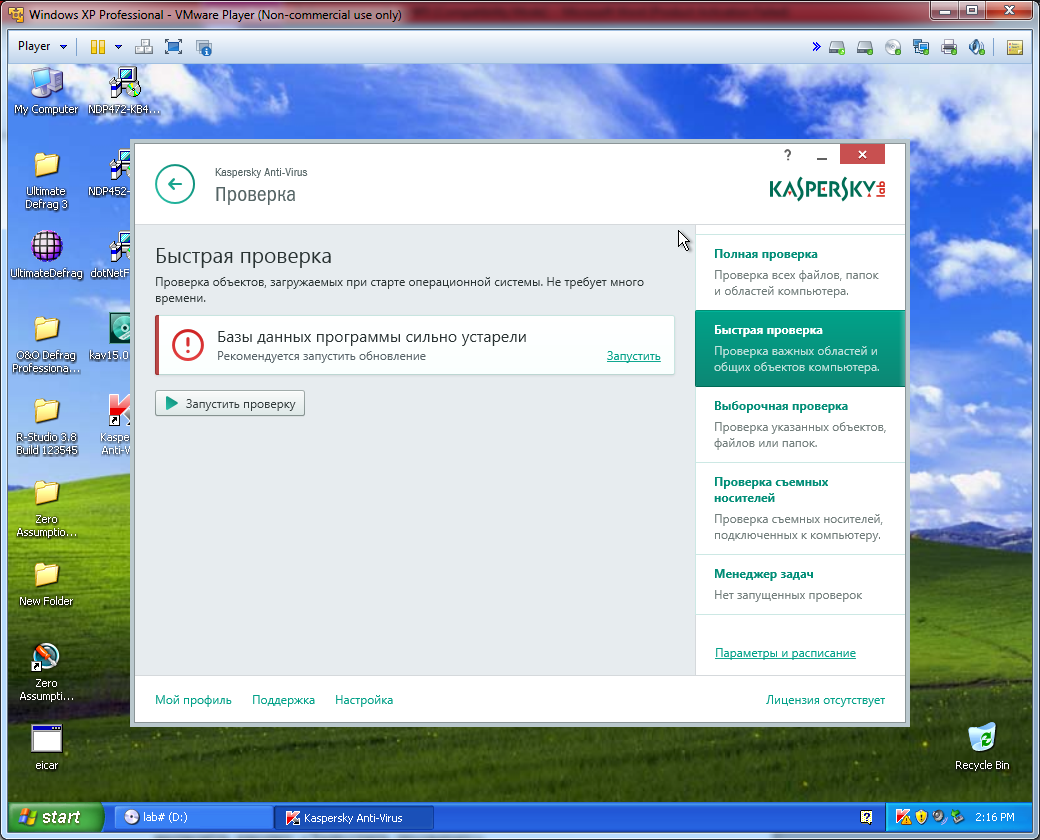
\includegraphics[height = 9\baselineskip]{./assets/y03s01-pcdiag-lab-05-p09.PNG}
				\caption{}
				\label{subfig:kaspersky-scan-quick}
			\end{subfigure}%
			\begin{subfigure}{0.5\textwidth}
				\centering
				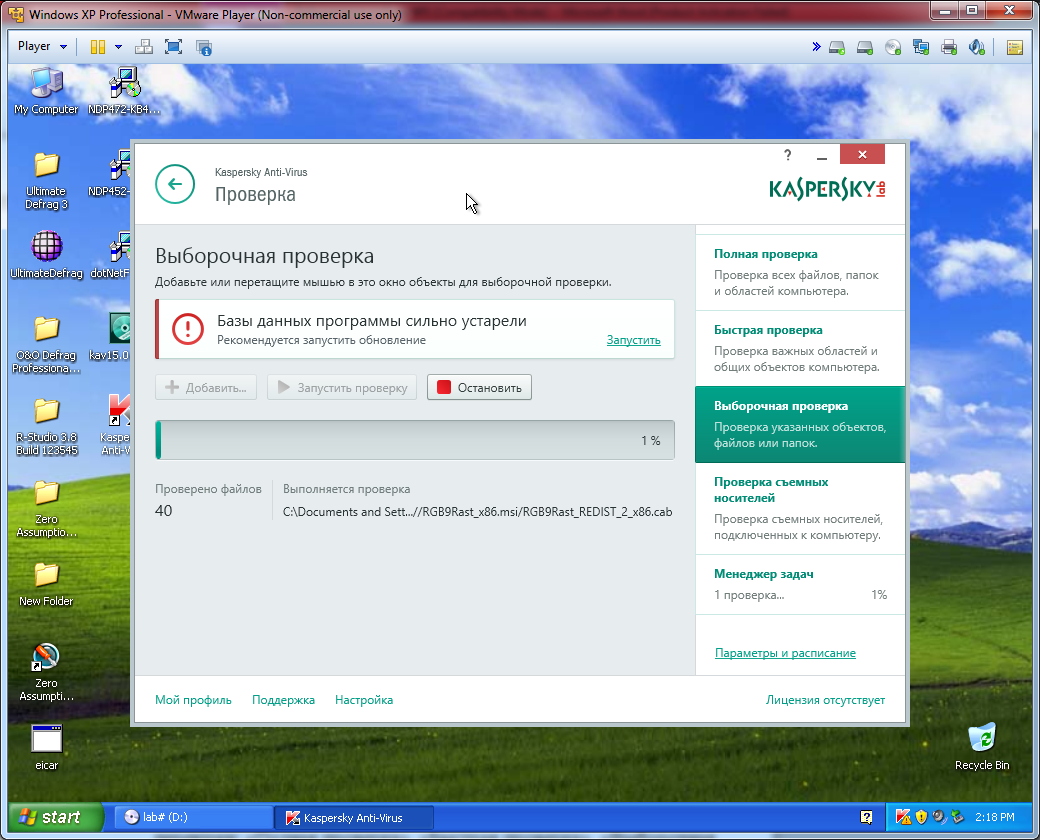
\includegraphics[height = 9\baselineskip]{./assets/y03s01-pcdiag-lab-05-p10.PNG}
				\caption{}
				\label{subfig:kaspersky-scan-selective-start}
			\end{subfigure}%
			\caption{Вікно запуску Швидкої та Вибіркової перевірок}
			\label{fig:kaspersky-scan-quick}
		\end{figure}

		Після завершення перевірки отримали результат: було знайдено 3~файли, які~антивірус вважає шкідливими~(рис.~\ref{fig:kaspersky-scan-results}). Антивірус не~пропонує жодних подальших дій зі~знайденими файлами, тому переглядаємо деталізацію.

		\begin{figure}[!htbp]
			\centering
			\begin{subfigure}{0.5\textwidth}
				\centering
				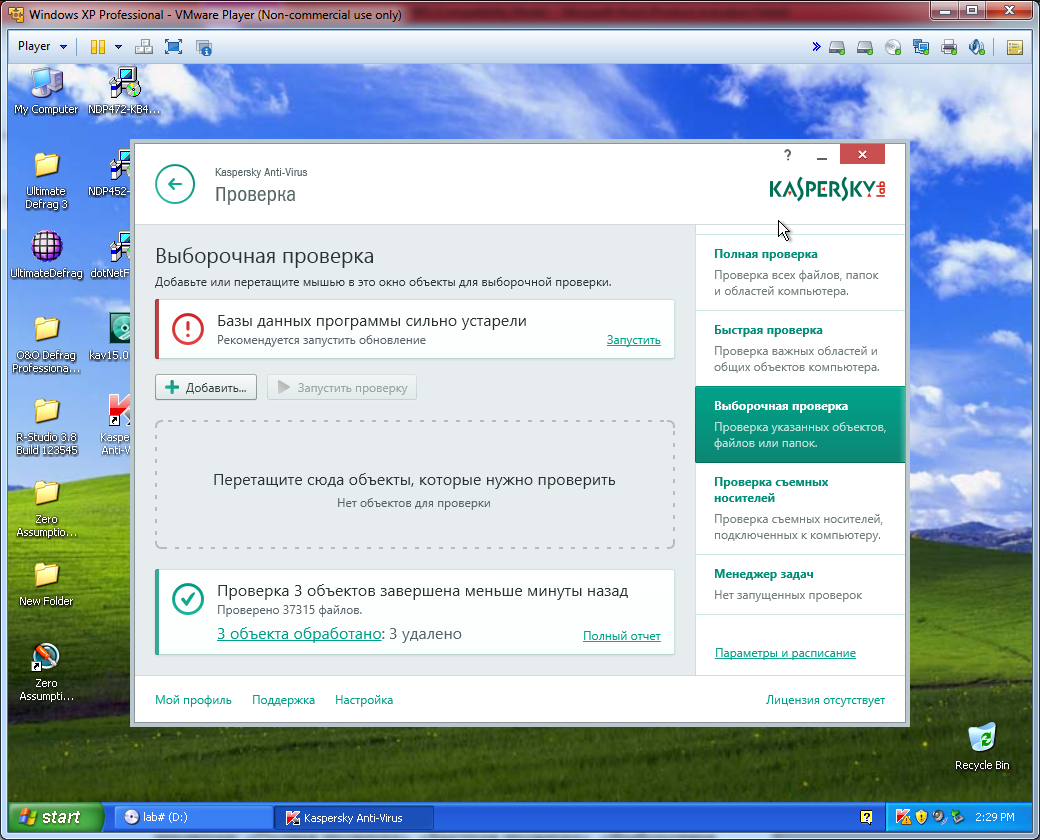
\includegraphics[height = 9\baselineskip]{./assets/y03s01-pcdiag-lab-05-p11.PNG}
				\caption{}
				\label{subfig:kaspersky-scan-results-summary}
			\end{subfigure}%
			\begin{subfigure}{0.5\textwidth}
				\centering
				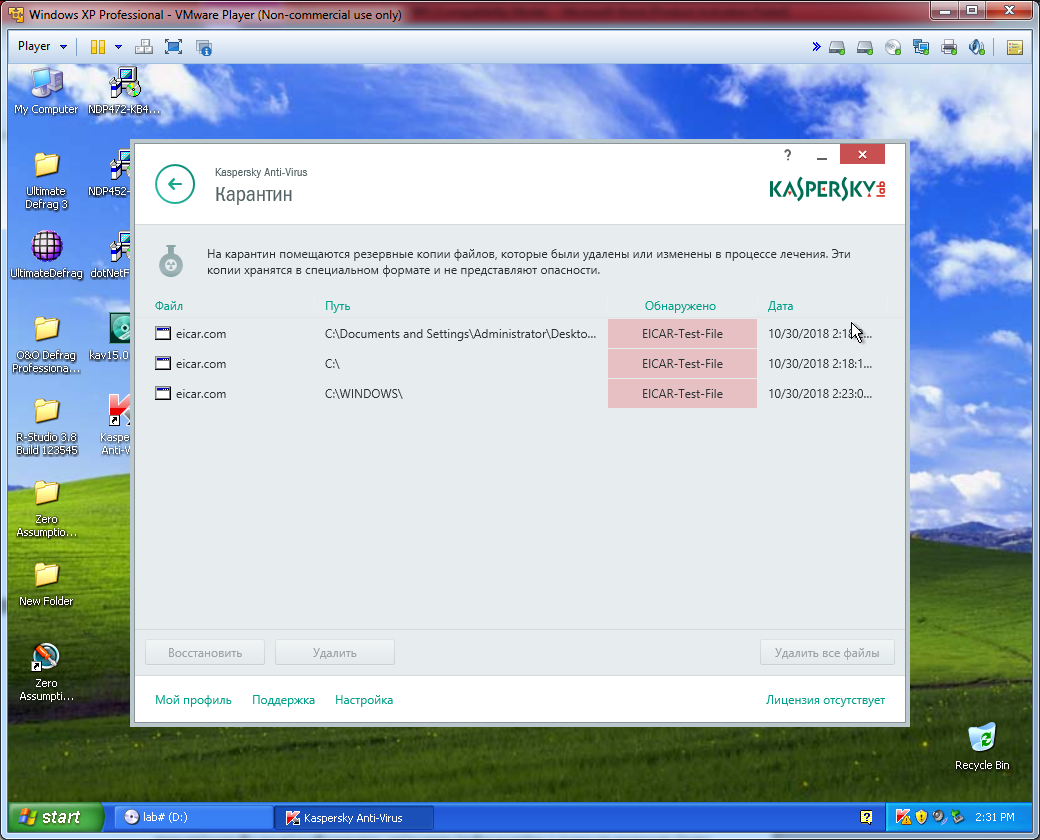
\includegraphics[height = 9\baselineskip]{./assets/y03s01-pcdiag-lab-05-p12.PNG}
				\caption{}
				\label{subfig:kaspersky-scan-results-details}
			\end{subfigure}%
			\caption{Результати перевірки комп'ютера на віруси}
			\label{fig:kaspersky-scan-results}
		\end{figure}

		Налаштовуємо параметри перевірки. Для~цього повертаємось у~головне меню, натискаємо кнопку «Налаштування» та~переходимо у~підпункт «Перевірка». В~обраному підпункті встановлюємо рівень безпеки «Рекомендований» та~дію при~знаходженні загрози~— «Лікувати, невиліковну~— видаляти»~(рис.~\ref{fig:kaspersky-settings}).

		\begin{figure}[!htbp]
			\centering
			\begin{subfigure}{0.5\textwidth}
				\centering
				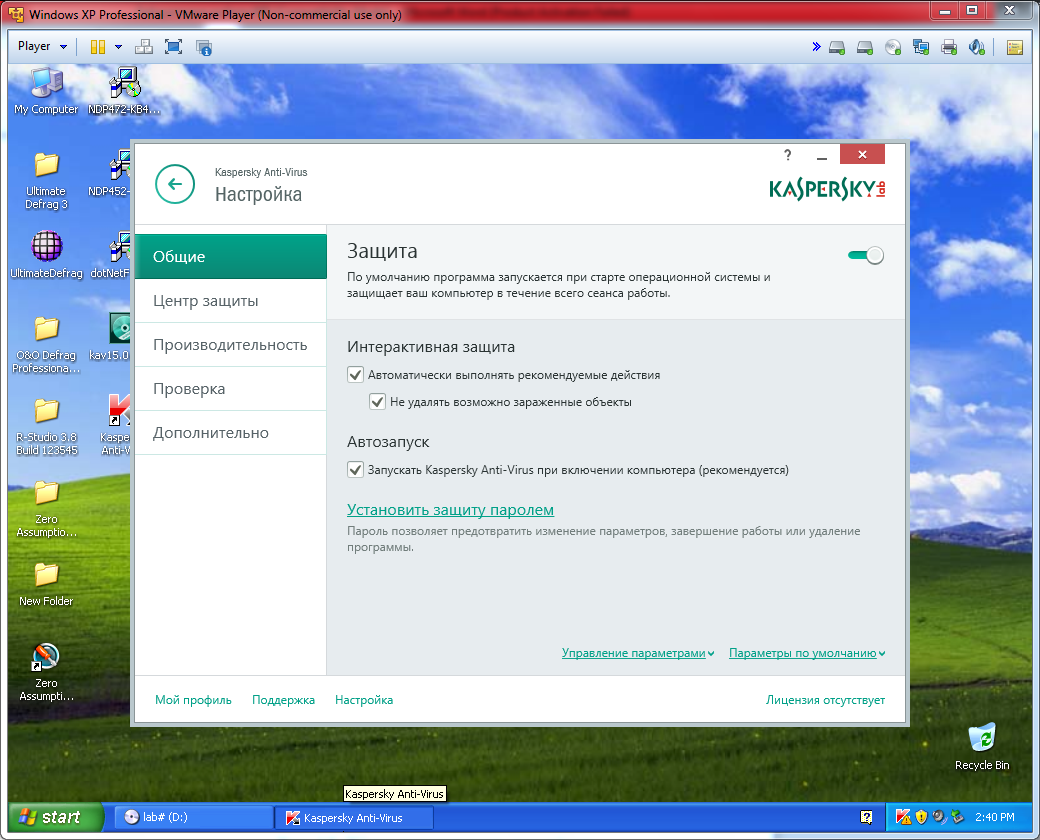
\includegraphics[height = 9\baselineskip]{./assets/y03s01-pcdiag-lab-05-p13.PNG}
				\caption{}
				\label{subfig:kaspersky-settings-general}
			\end{subfigure}%
			\begin{subfigure}{0.5\textwidth}
				\centering
				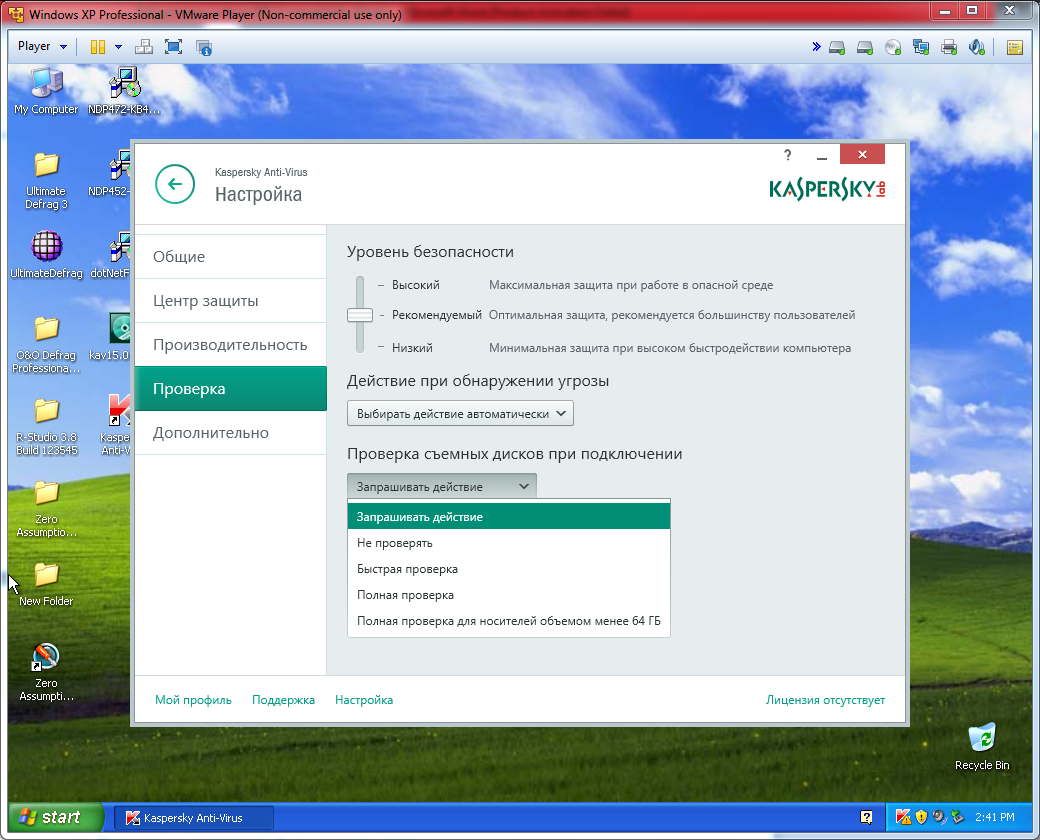
\includegraphics[height = 9\baselineskip]{./assets/y03s01-pcdiag-lab-05-p15.PNG}
				\caption{}
				\label{subfig:kaspersky-settings-scan}
			\end{subfigure}%
			\caption{Результати перевірки комп'ютера на віруси}
			\label{fig:kaspersky-settings}
		\end{figure}

	\section{Висновки}
		Виконуючи дану лабораторну роботу, ми ознайомились з~процесом використання антивірусного програмного забезпечення для~очищення комп'ютера від~вірусних загроз.

\end{document}
